%! Auswahl des Dokumententyps
%\documentclass[dissertation]{wbk}
\documentclass[oneside,studentpaper]{wbk}

%% Encoding: UTF-8 (direkte Verwendung von Umlauten etc.).
%% Die bib-Datei (BibTeX) wird trotzdem mit Escape-Zeichen formatiert.

%% Pakete
\usepackage{textcomp,amsmath,booktabs,microtype}
\usepackage{afterpage}
\usepackage{graphicx}
\usepackage{caption}
\captionsetup[figure]{labelfont=normalfont,textfont=normalfont}
\captionsetup[table]{labelfont=normalfont,textfont=normalfont,position=above}
\captionsetup[lstlisting]{labelfont=normalfont,textfont=normalfont,position=above}
\usepackage{float}
\usepackage{units}
\usepackage{tabularx}
\usepackage{cancel}
\usepackage{wrapfig}
\usepackage{longtable}
\usepackage{lscape}
\usepackage{enumitem}
\usepackage{amssymb}
\usepackage{multirow}
\usepackage{pdfpages}
\usepackage{tocloft}
\usepackage{icomma}
\usepackage{tikz}
\usetikzlibrary{arrows.meta,positioning,shapes.geometric,calc,backgrounds,fit}
\usepackage{subcaption}
\usepackage{underscore}
\usepackage{hyperref}
\usepackage{listings}
\usepackage{xcolor}

\definecolor{codegreen}{rgb}{0,0.6,0}
\definecolor{codegray}{rgb}{0.5,0.5,0.5}
\definecolor{codepurple}{rgb}{0.58,0,0.82}
\definecolor{backcolour}{rgb}{0.95,0.95,0.92}

% Farben fuer die TikZ-Diagramme
\definecolor{rgbblue}{rgb}{0.16,0.40,0.74}
\definecolor{rgbdteal}{rgb}{0.0,0.55,0.55}
\definecolor{shadowred}{rgb}{0.78,0.20,0.18}
\definecolor{boxgray}{rgb}{0.93,0.93,0.93}

% Einheitlicher Stil fuer ALLE Diagramme (Konsistenz ueber alle Abbildungen)
\tikzset{
  pipe/.style   ={rectangle, rounded corners=2pt, draw=black!55, fill=boxgray,
                  align=center, font=\small, minimum height=11mm,
                  minimum width=26mm, inner sep=3pt},
  pipeR/.style  ={pipe, fill=rgbblue!12,  draw=rgbblue!70},   % RGB
  pipeD/.style  ={pipe, fill=rgbdteal!14, draw=rgbdteal!70},  % RGB-D
  pipeS/.style  ={pipe, fill=shadowred!12, draw=shadowred!70},% Schatten / Loesung
  dec/.style    ={diamond, aspect=2.4, draw=shadowred!70, fill=shadowred!12,
                  align=center, font=\small, inner sep=1pt},
  flow/.style   ={-{Stealth[length=2.4mm]}, semithick, draw=black!70},
}

% Style-Optionen fuer Code-Listings
\lstdefinestyle{myStyle}{
    belowcaptionskip=1\baselineskip,
    breaklines=true,
    frame=none,
    numbers=none,
    basicstyle=\footnotesize\ttfamily,
    backgroundcolor=\color{backcolour},
    commentstyle=\itshape\color{codegreen},
    keywordstyle=\bfseries\color{magenta},
    numberstyle=\tiny\color{codegray},
    stringstyle=\color{codepurple},
}

% Einstellungen fuer Inkscape-Grafiken
\usepackage{transparent}
\graphicspath{{Abbildungen/}{Bilder/}{img/}}

\usepackage{chngcntr}
\counterwithout{footnote}{chapter}

\usepackage{mathtools}          % laedt amsmath ebenfalls
\DeclarePairedDelimiter\Floor\lfloor\rfloor
\DeclarePairedDelimiter\Ceil\lceil\rceil
\newlist{compactitem}{itemize}{3} % 3 = max-depth
\setlist[compactitem]{label=\textbullet, nosep}

\newcommand{\RM}[1]{\MakeUppercase{\romannumeral #1{}}}

% Alle Vektoren fett
\renewcommand{\vec}[1]{\boldsymbol{#1}}

%! Zwingend benoetigte Angaben.
	% Mehrere Autor:innen: bei Bedarf mit \\ stapeln, falls die Klasse das unterstuetzt.
	\author{Yannic Duan, Marc [Nachname], June [Nachname], Maximilian C. Klattig}
	\authorismale
	\title{Pose-Estimation in der Produktion}
	\subtitle{Seminararbeit -- Seminar \glqq KI in der Produktion\grqq}
	\placeanddate{Karlsruhe, \today}

	\birthplace{[Geburtsort]}
	\examdate{[TT.MM.JJJJ]}
	\mainreferent{[Pr\"ufer:in / Betreuer:in]}
	\coreferent{}
	\volumenum{}

%! Block nur bei Studentenarbeiten auszufuellen.
	\papertype{Seminararbeit}
	%% Sperrvermerke ggf. einkommentieren:
	%%\disclosuredate{}
	%%\disclosurecompany{}
	\matrnumber{[Matrikelnummer]}
	\authoraddress{[Adresse]}
	\handindate{[TT.MM.JJJJ]}
	\handoutdate{[TT.MM.JJJJ]}
	\papernumber{[FWT-XXXXXX]}

	\setlength{\bibsep}{\baselineskip} % Leerzeile zwischen Bibliographieeintraegen

\begin{document}
%? Sprache auswaehlen (die andere auskommentieren).
	\selectlanguage{ngerman}
	%\selectlanguage{english}

\maketitle

%! Block nur bei Dissertationen auszufuellen.
\ifDiss

	\begin{publisherpreface}
	\end{publisherpreface}

	\begin{authorpreface}
	\end{authorpreface}

%! Block nur bei Studentenarbeiten auszufuellen.
\else

	\newpage
	\thispagestyle{empty}
	\quad  \addtocounter{page}{-1}
	\newpage

%	\begin{disclosurenote}
%	\end{disclosurenote}

%! Eigenstaendigkeitserklaerung
	\statementoforiginality

%! Danksagung
	\begin{acknowledgment}
		% Hier Danksagung einfuegen.
	\end{acknowledgment}

%! Kurzzusammenfassung (Deutsch)
	\begin{summary}
		Diese Arbeit beschreibt ein Bildverarbeitungssystem, das aus einer
		einzelnen Aufnahme von oben die Lage von Metallbauteilen auf einer
		Montagetischplatte bestimmt, damit ein Roboterarm die Teile selbstständig
		greifen kann. Bestimmt werden für jedes Teil seine Position und seine
		Orientierung im Raum, zusammen als sechsdimensionale Lage bezeichnet.
		Sämtliche Trainings- und Testdaten werden in einer Simulation erzeugt und
		automatisch in das etablierte Auswertungsformat des BOP-Vergleichsstandards
		überführt. Untersucht und gegenübergestellt werden zwei Lösungswege: ein
		Weg über reine Farbbilder und ein Weg über Farbbilder mit zusätzlichem
		Tiefenkanal. Die Auswertung zeigt, dass der Farbbildweg die genaueste
		praktisch einsetzbare Lage liefert, während der Tiefenweg auf idealen
		Tiefendaten die höchste Genauigkeit überhaupt erreicht, im Schattenwurf des
		Roboterarms jedoch keine Tiefe mehr besitzt. Aus diesem komplementären
		Verhalten wird ein modulares System abgeleitet, das für jedes Bauteil
		anhand einer vorab berechneten Schattenkarte den jeweils geeigneten Weg
		auswählt.
	\end{summary}
\fi

%! Abstract (Englisch)
	\begin{abstract}
		This work presents a vision system that determines the pose of metallic
		parts on an assembly table from a single top-down image, enabling a robot
		arm to grasp the parts autonomously. For each part its position and
		orientation in space are estimated, jointly referred to as the
		six-dimensional pose. All training and test data are generated in
		simulation and automatically converted to the evaluation format of the BOP
		benchmark. Two approaches are compared: one using colour images only and
		one using colour images with an additional depth channel. The evaluation
		shows that the colour-image approach yields the most precise deployable
		pose, while the depth approach achieves the highest accuracy overall on
		ideal depth but loses all depth inside the shadow cast by the robot arm.
		From this complementary behaviour a modular system is derived that selects
		the suitable approach for each part based on a pre-computed shadow map.
	\end{abstract}

%! Einstellungen fuer LOF und LOT
\setlength{\cftbeforeloftitleskip}{12pt}
\addtocontents{lof}{\begin{flushright}
		\textbf{Seite}
	\end{flushright}\par}

\setlength{\cftbeforelottitleskip}{12pt}
\addtocontents{lot}{\begin{flushright}
		\textbf{Seite}
	\end{flushright}\par}

% Einleitende Kapitel im frontmatter, Seiten roemisch nummeriert.
\frontmatter

\tocloftpagestyle{empty}
\setlength{\cftbeforetoctitleskip}{12pt}
\addtocontents{toc}{\protect\setcounter{tocdepth}{-1}}
\tableofcontents
\addtocontents{toc}{\begin{flushright}
		\textbf{Seite}
	\end{flushright}\par}
\addtocontents{toc}{\protect\setcounter{tocdepth}{2}}

%! Abkuerzungsverzeichnis
\chapter{Abk\"urzungen}

\begin{longtable}{p{3cm} p{13cm}}
	\textbf{Abk\"urzung} & \textbf{Beschreibung} \\ \midrule \endhead
	AABB    & achsenparalleles umschlie{\ss}endes Rechteck (Axis-Aligned Bounding Box) \\
	AR      & Average Recall (Hauptkennzahl des BOP-Vergleichs) \\
	BOP     & Benchmark for 6D Object Pose Estimation (Vergleichsstandard) \\
	CAD     & rechnergest\"utzte Konstruktion (Computer-Aided Design) \\
	ICP     & Iterative-Closest-Point-Verfahren \\
	IR      & Infrarot \\
	MoE     & Mixture of Experts (Expertenauswahl) \\
	MSPD    & symmetriebewusster 2D-Projektionsabstand \\
	MSSD    & symmetriebewusster 3D-Oberfl\"achenabstand \\
	OBB     & orientiertes umschlie{\ss}endes Rechteck (Oriented Bounding Box) \\
	PBR     & physikalisch basiertes Rendern (Physically Based Rendering) \\
	RGB     & Farbbild (Rot-Gr\"un-Blau) \\
	RGB-D   & Farbbild mit zus\"atzlichem Tiefenkanal \\
	SDG     & synthetische Datenerzeugung (Synthetic Data Generation) \\
\end{longtable}

\cleardoublepage

%! Formelzeichenverzeichnis
\begin{longtable}{l p{0.56\textwidth} l l}
	\textbf{Formelzeichen} & \textbf{Beschreibung} & \textbf{Einheit} & \textbf{Wertebereich} \\ \midrule \endhead
	$\vec{R}$ & Rotationsmatrix Objekt zur Welt & -- & $SO(3)$ \\
	$\vec{t}$ & Translationsvektor (Objektzentrum) & mm & -- \\
	$\vec{K}$ & Kamera-Intrinsik-Matrix & -- & -- \\
	$\theta$ & MSSD-Schwelle ($0{,}1 \cdot$ Durchmesser) & mm & $\approx 11$ \\
	$d$ & Objektdurchmesser & mm & -- \\
	$z_w$ & H\"ohe \"uber der Tischebene & mm & $\geq 0$ \\
\end{longtable}

% Hauptteil im mainmatter. Hier beginnen die eigentlichen Seitenzahlen.
\mainmatter

% ====================================================================
\chapter{Einleitung}
% ====================================================================

In einer automatisierten Montagezelle soll ein Roboterarm Metallbauteile von
einer Tischplatte selbstständig aufnehmen. Dafür muss das System nicht nur
erkennen, welche Teile auf dem Tisch liegen, sondern auch, an welcher Stelle und
in welcher Drehlage. Position und Orientierung eines Teils werden gemeinsam als
sechsdimensionale Lage bezeichnet, weil drei Koordinaten die Position und drei
weitere die Drehung beschreiben. Eine reine Erkennung der Teile in der Bildebene
genügt für einen sicheren Griff nicht, da der Greifer die vollständige Lage im
Raum benötigt.

Die Konstruktionsdaten aller Bauteile liegen als CAD-Modelle vor. Was bislang
fehlte, war die Bildverarbeitung, die diese Modelle mit einer Kameraaufnahme der
Zelle verbindet und daraus die Lage jedes Teils ableitet. Die Aufgabe ist
anspruchsvoll, weil es sich um glänzende, weitgehend texturlose Metallteile mit
ausgeprägten Drehsymmetrien handelt. Solche Teile werden unter wechselnder
Beleuchtung aufgenommen und teilweise durch den Roboterarm selbst verdeckt.

Ziel der Arbeit ist ein System, das aus einer einzelnen Aufnahme von oben die
liegenden, bekannten Bauteile bestimmt und ihre Lage so genau schätzt, dass die
Teile anschließend als CAD-Modell an der richtigen Stelle in einem
3D-Betrachter dargestellt und vom Roboter gegriffen werden können. Die Bewertung
der Genauigkeit erfolgt durchgängig nach dem BOP-Vergleichsstandard, dem
etablierten Maßstab für die Lageschätzung von Objekten \cite{bop2024}. Alle
benötigten Daten werden in einer Simulation erzeugt. Das vermeidet die aufwändige
und fehleranfällige Vermessung realer Aufnahmen und liefert beliebig viele Szenen
mit exakt bekannter Referenzlage.

Die Arbeit gliedert sich nach einer Einordnung in den Stand der Technik in eine
Problemstellung, die die Aufgabe und ihre Randbedingungen präzise fasst, in die
Methodik mit der Datenerzeugung und den beiden untersuchten Lösungswegen
(Kapitel~\ref{ch:methodik}) sowie in die daraus entwickelte Lösung in Form eines
modularen Systems (Kapitel~\ref{ch:loesung}). Die zentrale Erkenntnis lässt sich
vorwegnehmen: Farbbild und Tiefenbild stehen nicht in Konkurrenz, sondern
ergänzen sich örtlich. Der Tiefenweg ist genauer, wo verlässliche Tiefe vorliegt;
im Schatten des Roboterarms ist allein der Farbweg verwertbar. Genau diese
Aufteilung nutzt das entwickelte System.

% ====================================================================
\chapter{Stand der Forschung}
\label{ch:stand}
% ====================================================================

\section{Der BOP-Vergleichsstandard und seine Kennzahlen}

Der BOP-Vergleichsstandard \cite{bop2024} legt das Datenformat, die Datensätze
und die Auswertung für die Lageschätzung von Objekten fest. Die Hauptkennzahl ist
der Average Recall (AR). Er gibt vereinfacht den Anteil der Schätzungen an, deren
Lagefehler unter einer festgelegten Schwelle bleibt, gemittelt über drei
Fehlermaße. Diese drei Maße betrachten den Fehler aus verschiedenen Blickwinkeln:
als Tiefenabweichung der sichtbaren Oberfläche (VSD), als dreidimensionalen
Oberflächenabstand (MSSD) und als zweidimensionalen Projektionsabstand in der
Bildebene (MSPD). Für symmetrische Objekte ist entscheidend, dass MSSD und MSPD
den Fehler über alle erlaubten Symmetrielagen des Objekts minimieren. Eine
korrekte Lage wird so nicht fälschlich als Fehler gewertet, nur weil das Teil um
eine Symmetrieachse verdreht erscheint. Die Referenzimplementierung dieser
Kennzahlen stellt das frei verfügbare \texttt{bop\_toolkit} bereit
\cite{boptoolkit}.

\section{Farbbild- gegenüber Tiefenverfahren}

Verfahren zur Lageschätzung lassen sich grob danach einteilen, ob sie nur das
Farbbild verwenden oder zusätzlich ein Tiefenbild. Ein Tiefenbild liefert für
jeden Bildpunkt seinen Abstand zur Kamera und damit die metrische Größe der Szene
unmittelbar. Reine Farbverfahren müssen diese Größe dagegen aus dem Erscheinungsbild
erschließen. Auf den Bestenlisten des BOP-Vergleichs liegen die genauesten
Verfahren durchgängig auf der Tiefenseite, und reine Farbverfahren liegen
spürbar, in der Größenordnung von rund 20 Prozentpunkten, darunter
\cite{bop2024}. Diesem Vorteil steht ein praktischer Nachteil gegenüber: Auf
glänzendem Metall ist das Tiefenbild durch Reflexionen verrauscht, sodass die
nominelle Stärke der Tiefe in der Anwendung teilweise verloren geht.

\section{Verwendete Verfahren}

Tabelle~\ref{tab:methoden} fasst die Bausteine zusammen, auf denen diese Arbeit
aufbaut. Für den Farbweg ist GDRNPP \cite{gdrnpp2025} maßgeblich, das
Gewinnerverfahren des BOP-Vergleichs von 2022 und eine Weiterentwicklung von
GDR-Net \cite{gdrnet2021}. GDRNPP wird je Bauteil eigens trainiert und erreicht
auf synthetischen Daten eine hohe Genauigkeit. Die Bauteile im Bild findet ein
YOLOv8-Detektor mit orientierten Rechtecken \cite{yolov8}.

Für den Tiefenweg werden Verfahren eingesetzt, die ohne bauteilspezifisches
Training auskommen und sich daher direkt auf neue Teile übertragen lassen. Solche
Verfahren werden als trainingsfrei für das jeweilige Objekt bezeichnet. Dazu
gehören FoundationPose \cite{foundationpose2024}, das eine Lage durch
wiederholtes Rendern und Vergleichen mit dem Tiefenbild verfeinert und unter den
führenden Verfahren des BOP-Vergleichs von 2024 lag, sowie GigaPose
\cite{gigapose2024}, das aus einer einzelnen Bildkorrespondenz schnell eine
Grobschätzung gewinnt und diese im Tiefenmodus an die Tiefendaten anpasst. Das
zugehörige Erkennungsökosystem bilden CNOS \cite{cnos2023}, das
Segmentierungsmodell Segment Anything \cite{sam2023} und der Bildbeschreiber
DINOv2 \cite{dinov2_2023}; MegaPose \cite{megapose2022} dient als Verfeinerer der
trainingsfreien Linie. Die synthetischen Daten erzeugt NVIDIA Isaac Sim
\cite{isaacsim}.

\begin{table}[H]
\caption{Verwendete Verfahren, geordnet nach Rolle. Die Spalte Training
unterscheidet bauteilspezifisch trainierte von trainingsfreien Verfahren.}
\label{tab:methoden}
\centering
\small
\begin{tabularx}{\textwidth}{l l l l X}
\toprule
\textbf{Verfahren} & \textbf{Rolle} & \textbf{Modalität} & \textbf{Training} & \textbf{Lizenz} \\
\midrule
YOLOv8-OBB      & Erkennung        & RGB    & trainiert       & AGPL-3.0 \\
GDRNPP          & Lage (Farbe)     & RGB    & je Bauteil      & Apache-2.0 \\
GigaPose        & Lage (grob)      & RGB / RGB-D & trainingsfrei & MIT \\
FoundationPose  & Lage (Tiefe)     & RGB-D  & trainingsfrei   & NVIDIA (nicht kommerziell) \\
CNOS / SAM      & Erkennung        & RGB    & trainingsfrei   & MIT / Apache-2.0 \\
MegaPose        & Verfeinerung     & RGB / RGB-D & trainingsfrei & Apache-2.0 \\
\texttt{bop\_toolkit} & Kennzahlen & --     & --              & MIT \\
Isaac Sim       & Datenerzeugung   & --     & --              & proprietär \\
\bottomrule
\end{tabularx}
\end{table}

% ====================================================================
\chapter{Problemstellung}
\label{ch:problem}
% ====================================================================

Aus der Anwendung und dem Stand der Technik ergibt sich eine klar umrissene
Aufgabe. Gesucht ist die sechsdimensionale Lage jedes bekannten Bauteils auf
einer Tischplatte, ermittelt aus einer einzelnen Aufnahme von oben, mit einer
Genauigkeit, die einen sicheren Robotergriff erlaubt. Die Konstruktionsdaten der
Teile liegen vor, und die Teile ruhen auf einer bekannten, ebenen Tischfläche.

Mehrere Randbedingungen erschweren die Aufgabe und prägen die Lösung. Die
Bauteile sind glänzend und weitgehend texturlos, weshalb sich kaum
wiedererkennbare Bildmerkmale auf ihrer Oberfläche befinden. Mehrere Teile
besitzen eine Drehsymmetrie, sodass aus einem einzelnen Bild grundsätzlich
mehrere Drehlagen gleich gut zum Bild passen können. Der Roboterarm steht im Bild
und verdeckt Teile sowohl optisch als auch im Tiefenbild. Schließlich liefert ein
reales Tiefenbild auf glänzendem Metall verrauschte Werte, weshalb nicht von
vornherein feststeht, ob die zusätzliche Tiefe in der Anwendung tatsächlich
nützt.

Daraus ergibt sich der Kern der Untersuchung. Ein Farbweg verzichtet auf die
unsichere Tiefe, muss die fehlende metrische Größe aber anderweitig gewinnen. Ein
Tiefenweg nutzt die Tiefe direkt, hängt jedoch von deren Qualität und
Verfügbarkeit ab. Es ist nicht im Voraus klar, welcher Weg in dieser konkreten
Umgebung überlegen ist und ob ein einzelner Weg überhaupt für alle Stellen der
Tischfläche genügt. Die Arbeit beantwortet diese Frage in drei Schritten: Sie
erzeugt eine geeignete Datengrundlage, sie baut beide Wege getrennt auf und reizt
sie aus, und sie leitet aus dem Vergleich eine Lösung ab, die die Stärken beider
Wege verbindet.

% ====================================================================
\chapter{Methodik}
\label{ch:methodik}
% ====================================================================

\section{Gesamtvorgehen}

Das Vorgehen umfasst vier Stufen, die Abbildung~\ref{fig:overview} zeigt. Zuerst
werden die Daten der Montagezelle simuliert und in das BOP-Format überführt.
Darauf aufbauend werden zwei getrennte Wege bereitgestellt, ein Farbweg und ein
Tiefenweg. Beide Wege werden unter demselben Auswertungsverfahren bewertet, damit
der Vergleich aussagekräftig ist. Aus dem Vergleich folgt schließlich die
Lösung, die in Kapitel~\ref{ch:loesung} beschrieben wird. Beide Wege wurden
bewusst zunächst getrennt bis an ihre Grenze optimiert, denn nur so lässt sich
beziffern, was jeder Weg für sich leistet und unter welchen Bedingungen er
versagt.

\begin{figure}[H]
\centering
\begin{tikzpicture}[node distance=7mm and 9mm]
  \node[pipe]                       (sim)   {Daten-\\simulation};
  \node[pipe, right=of sim]         (train) {Modelle\\bereitstellen};
  \node[pipeR, right=of train]      (rgb)   {Farbweg\\(GDRNPP)};
  \node[pipeD, below=6mm of rgb]    (rgbd)  {Tiefenweg\\(FoundationPose,\\GigaPose-3D)};
  \node[pipe, right=11mm of rgb, minimum height=20mm, yshift=-9mm] (eval) {Bewertung\\(BOP)};
  \node[pipeS, right=of eval, minimum height=20mm] (loes) {Lösung\\(Kap.~\ref{ch:loesung})};
  \draw[flow] (sim) -- (train);
  \draw[flow] (train.east) -- ++(4mm,0) |- (rgb.west);
  \draw[flow] (train.east) -- ++(4mm,0) |- (rgbd.west);
  \draw[flow] (rgb.east)  -| (eval.north);
  \draw[flow] (rgbd.east) -| (eval.south);
  \draw[flow] (eval) -- (loes);
\end{tikzpicture}
\caption{Gesamtvorgehen mit vier Stufen: synthetische Daten, zwei getrennt
optimierte Wege, einheitliche Bewertung und die daraus abgeleitete Lösung.}
\label{fig:overview}
\end{figure}

\section{Datensimulation und BOP-Konvertierung}
\label{sec:datasim}

Statt reale Aufnahmen aufwändig von Hand mit ihrer Referenzlage zu versehen, wird
die Montagezelle vollständig in NVIDIA Isaac Sim gerendert \cite{isaacsim}. Die
Simulation liefert beliebig viele Szenen mit exakt bekannter Lage, Maske, Tiefe
und Begrenzungsrechteck und erlaubt eine kostenlose Variation von Beleuchtung,
Material und Anordnung der Teile.

Gerendert wird eine Aufnahme von oben mit sichtbarem Roboterarm. Dies entspricht
der realen Situation, in der der Arm ebenfalls im Bild steht und Teile verdeckt.
Die Bauteile werden in der Simulation physikalisch auf den Tisch fallen gelassen,
sodass sie in natürlichen Ruhelagen liegen. Beleuchtung, Materialeigenschaften,
Kameraschwankungen und Anordnung werden dabei zufällig variiert. Diese
Variation ist gerade auf texturlosem Metall der wirksamste Hebel, damit ein in
der Simulation trainiertes Modell später auf realen Bildern funktioniert
\cite{thalhammer2024}.

Isaac Sim kann nicht unmittelbar im BOP-Format schreiben. Daher wurde ein eigener
Konverter erstellt, der den Simulationsausgang in die BOP-Struktur überführt; den
Ablauf zeigt Abbildung~\ref{fig:datapipe}. Erzeugt werden die Beschreibungen der
Szene und der Kamera sowie ein Verzeichnis mit den CAD-Modellen in Millimeter und
einer Datei mit Durchmesser und Symmetrieangaben je Bauteil. Die Symmetrien sind
für die Anker und den Ringmagnet eine durchgehende Drehbarkeit um die Längsachse
und für das Zahnrad eine siebenzählige Symmetrie. Falsche Symmetrieangaben würden
den Drehfehler künstlich erhöhen; ihre korrekte Angabe ist daher Voraussetzung
für eine faire Bewertung.

Eine zunächst unscheinbare, für den Tiefenweg aber folgenreiche Festlegung
betrifft die Bedeutung der Tiefenwerte. Die Simulation liefert den Abstand
entlang des Sehstrahls, während die nachgelagerten Verfahren den senkrechten
Abstand zur Bildebene erwarten. Werden die Werte unverändert übernommen, entsteht
ein systematischer Tiefenfehler, der zum Bildrand hin wächst. Der Konverter
rechnet die Werte deshalb in den senkrechten Abstand um. Welche Wirkung dieses
Detail hatte, wird in Abschnitt~\ref{sec:fairness} beziffert.

\begin{figure}[H]
\centering
\begin{tikzpicture}[node distance=6mm and 8mm]
  \node[pipe]                    (cad)    {CAD-Modell};
  \node[pipe, right=of cad]      (cell)   {Isaac-Zelle\\(Aufnahme von oben,\\Arm sichtbar)};
  \node[pipe, right=of cell]     (conv)   {Konverter\\(senkrechte Tiefe)};
  \node[pipe, right=of conv]     (bop)    {BOP-Datensatz\\(Training / Test)};
  \node[pipe, below=7mm of conv] (models) {Modelle in mm\\und Symmetrien};
  \draw[flow] (cad) -- (cell);
  \draw[flow] (cell) -- (conv);
  \draw[flow] (conv) -- (bop);
  \draw[flow] (cad.south) |- (models.west);
  \draw[flow] (models.east) -| (bop.south);
\end{tikzpicture}
\caption{Datenpipeline: aus dem CAD-Modell und der gerenderten Zelle entsteht ein
BOP-Datensatz mit korrekten Modellen und Symmetrieangaben.}
\label{fig:datapipe}
\end{figure}

\section{Farbweg}
\label{sec:rgb}

Die ursprüngliche Festlegung war ein reiner Farbweg ohne Tiefe, weil reale
Tiefendaten auf den glänzenden Metallteilen durch Reflexionen unzuverlässig sind
und das System nicht auf instabile Tiefenwerte gestützt werden sollte. Der dadurch
zu erwartende Genauigkeitsnachteil wird durch eine geometrische Zusatzbedingung
teilweise ausgeglichen: Da die Teile auf einer bekannten, ebenen Tischfläche
ruhen, reduziert sich die eigentlich sechsdimensionale Aufgabe näherungsweise auf
die Lage in dieser Ebene.

Von den untersuchten Varianten wird hier nur die stärkste und praktisch
einsetzbare Kombination beschrieben, im Folgenden als Pipeline~A bezeichnet. Sie
besteht aus drei Schritten, die Abbildung~\ref{fig:rgbpipe} zeigt. Zunächst findet
der YOLOv8-Detektor die Bauteile im Bild und liefert orientierte Rechtecke um die
Teile. Aus diesen werden achsenparallele Bildausschnitte erzeugt, wie sie GDRNPP
benötigt. Anschließend schätzt für jede Bauteilklasse ein eigenes, in der
Simulation trainiertes GDRNPP-Modell aus dem Farbausschnitt die Lage. Zuletzt
überführt ein Adapter die geschätzte Lage in das Weltkoordinatensystem mit dem
Tischnullpunkt als Ursprung, vereinheitlicht die Symmetrie und setzt das Teil
über die Tischebenenbedingung sauber auf die Tischfläche auf.

\begin{figure}[H]
\centering
\begin{tikzpicture}[node distance=8mm]
  \node[pipeR]                 (img)   {Farbbild\\von oben};
  \node[pipeR, right=of img]   (det)   {Erkennung\\(YOLOv8-OBB)};
  \node[pipeR, right=of det]   (pose)  {Lage je Bauteil\\(GDRNPP)};
  \node[pipeR, right=of pose]  (world) {Welt-Lage\\und Aufsetzen};
  \node[pipeR, right=of world] (view)  {3D-Betrachter};
  \draw[flow] (img) -- (det);
  \draw[flow] (det) -- (pose);
  \draw[flow] (pose) -- (world);
  \draw[flow] (world) -- (view);
\end{tikzpicture}
\caption{Farbweg (Pipeline~A): Erkennung, bauteilweise Lageschätzung mit GDRNPP
und Überführung in die Weltlage mit Aufsetzen auf die Tischebene.}
\label{fig:rgbpipe}
\end{figure}

Pipeline~A erreicht auf den beiden Ankerklassen einen Average Recall von 0,886.
Die bauteilweisen Modelle erzielen einzeln 0,870 für den kurzen Anker, 0,907 für
den langen Anker und 0,838 für das Zahnrad. Der Translationsfehler liegt im Mittel
bei rund vier Millimeter, was die Schätzung sehr genau macht. Der entscheidende
Grund dafür ist das bauteilspezifische Training.

Der Farbweg bietet die höchste praktisch einsetzbare Genauigkeit und ist gegen
verrauschte Tiefenbilder robust, da er gar keine Tiefe verwendet. Die eingesetzten
Komponenten der Lageschätzung sind freizügig lizenziert, und die Laufzeit ist
gering. Dem steht gegenüber, dass jedes Bauteil ein eigenes trainiertes Modell
benötigt und der Weg sich daher nicht ohne Weiteres auf unbekannte Teile
übertragen lässt. Außerdem wird die fehlende metrische Tiefe nur über die
Tischebenenbedingung erschlossen, die außerhalb der Ebene nicht trägt.

\section{Tiefenweg}
\label{sec:rgbd}

Der Reiz des Tiefenwegs liegt darin, dass das Tiefenbild die metrische Größe
unmittelbar liefert, also genau jene Information, die der Farbweg erst erschließen
muss. Zudem arbeiten die hier eingesetzten Verfahren ohne bauteilspezifisches
Training, sodass sich die Lageschätzung ohne weiteren Trainingsaufwand auf neue
Teile übertragen ließe.

Untersucht wurden zwei Tiefenverfahren auf denselben Erkennungen wie Pipeline~A.
FoundationPose dient als obere Genauigkeitsgrenze, da es eine Lage durch
wiederholtes Rendern und Abgleichen mit dem Tiefenbild verfeinert. GigaPose im
Tiefenmodus dient als lizenzrechtlich unbedenkliche und damit einsetzbare
Variante. Beide Verfahren verwenden die in Abschnitt~\ref{sec:datasim}
beschriebene, in den senkrechten Abstand umgerechnete Tiefe.

Auf der idealen Tiefe der Simulation erreicht FoundationPose mit einem Average
Recall von 0,968 den höchsten Wert aller untersuchten Verfahren und übertrifft
damit den trainierten Farbweg. GigaPose im Tiefenmodus erreicht 0,838. Der
scheinbare Widerspruch zur Aussage, der Farbweg sei genauer, klärt sich über zwei
Punkte, die die folgenden Abschnitte ausführen: zum einen über die zuvor genannte
Tiefenkonvention (Abschnitt~\ref{sec:fairness}), zum anderen über den Unterschied
zwischen idealer Tiefe aus der Simulation und verrauschter Tiefe in der Realität.

Eine genauere Betrachtung des verbleibenden Fehlers
(Abschnitt~\ref{sec:rgbd-charakter}) zeigt, dass es sich nicht um einen
systematischen Versatz und nicht um einen Symmetriefehler handelt, sondern um ein
zufälliges Schwanken der Schätzung von rund 30 bis 48 Millimeter. Dieses Schwanken
ist eine Eigenschaft der trainingsfreien Verfeinerung auf den schlichten, nahezu
quaderförmigen Ankerausschnitten und liegt deutlich über den rund vier Millimeter
des bauteilspezifisch trainierten Farbwegs.

Der Tiefenweg benötigt kein bauteilspezifisches Training und liefert die
metrische Tiefe unmittelbar, was auf idealer Tiefe die höchste Genauigkeit
überhaupt ermöglicht. Seine Schwäche ist die Abhängigkeit von der Qualität des
Tiefenbildes. Auf glänzendem Metall ist diese verrauscht, und im Schatten des
Arms fehlt die Tiefe vollständig. Hinzu kommt, dass das genaueste Verfahren,
FoundationPose, nur unter einer nicht-kommerziellen Lizenz nutzbar und mit rund
acht Sekunden je Bild langsam ist.

\section{Bewertungsverfahren}
\label{sec:evalmethodik}

Beide Wege werden unter demselben Verfahren bewertet, damit der Vergleich
belastbar ist. Verwendet werden dieselben gerenderten Testszenen, dieselben
Kameradaten für Schätzung und Bewertung und dieselbe symmetriebewusste Kennzahl
aus dem \texttt{bop\_toolkit} \cite{boptoolkit}. Die maßgebliche Zahl ist der
Average Recall auf den beiden Ankerklassen über jeweils 100 Szenen. Die Schwelle
des dreidimensionalen Oberflächenmaßes beträgt ein Zehntel des Objektdurchmessers
und liegt damit bei etwa elf Millimeter. Die durchgehende Drehsymmetrie der Anker
wird bei der Bewertung herausgerechnet, sodass der dem Auge zunächst große
Drehfehler durch das Verdrehen um die Längsachse korrekt auf wenige Grad
zusammenfällt. Das Aufsetzen auf die Tischebene ist bei der Bewertung
abgeschaltet, um die reine Schätzgenauigkeit zu messen.

\section{Faire Vergleichsbedingungen}
\label{sec:fairness}

Über mehrere Schritte erschien der Tiefenweg systematisch schlechter als der
Farbweg. Die Ursache war kein Nachteil der Verfahren, sondern die in
Abschnitt~\ref{sec:datasim} genannte Tiefenkonvention. Der Abstand entlang des
Sehstrahls wurde als senkrechter Abstand zur Bildebene gedeutet, was alle
tiefenverarbeitenden Verfahren mit einem zum Bildrand wachsenden Fehler belastete.
Der gemessene mittlere Fehler betrug rund 38 Millimeter, und eine geometrische
Vorhersage dieses Fehlers stimmte mit den Messwerten sehr gut überein. Nach der
Korrektur sank der Fehler auf rund sechs Millimeter. Erst diese Korrektur stellte
faire Bedingungen her, und sie kehrte das Bild um, denn der trainingsfreie
Tiefenweg mit FoundationPose und 0,968 übertraf nun den trainierten Farbweg mit
0,886. Die methodische Lehre daraus ist, bei einem gleichartigen Fehler einer
ganzen Verfahrensgruppe zuerst die Datengrundlage zu prüfen, bevor man eine Grenze
der Verfahren annimmt.

\section{Charakter des verbleibenden Tiefenfehlers}
\label{sec:rgbd-charakter}

Nach der Korrektur bleibt eine echte Genauigkeitslücke der einsetzbaren
Tiefenvariante gegenüber dem trainierten Farbweg. Eine gezielte Untersuchung
schließt zwei naheliegende Ursachen aus, wie Tabelle~\ref{tab:rgbd-fehler} zeigt.
Erstens wird die Symmetrie korrekt herausgerechnet. Der dem Auge große Drehfehler
der Anker von rund 77 Grad, der nur das Verdrehen um die Längsachse beschreibt,
fällt symmetriebereinigt auf wenige Grad zusammen. FoundationPose erreicht dabei
5,0 Grad und liegt damit sogar leicht besser als GDRNPP mit 7,2 Grad, während
GigaPose im Tiefenmodus mit 15,2 Grad etwas darüber liegt, aber weit unter dem
unbereinigten Wert. Die Drehung ist also nicht die Schwäche der trainingsfreien
Verfahren. Zweitens gibt es keinen festen Versatz im Modell, denn der mittlere
Lagefehler ist nahezu null bei großer und richtungsloser Streuung. Es gibt damit
nichts anzugleichen.

Der verbleibende Fehler ist ein zufälliges Schwanken der trainingsfreien
Verfeinerung von rund 30 bis 48 Millimeter, gegenüber rund vier Millimeter beim
bauteilspezifisch trainierten Farbweg. Dieses Schwanken liegt über der Schwelle
des dreidimensionalen Maßes von etwa elf Millimeter, weshalb die Genauigkeit nach
diesem Maß einbricht, während das zweidimensionale Projektionsmaß bei rund 0,97
bleibt, weil die Drehung korrekt ist und dieses Maß gegen Tiefenfehler
unempfindlich ist. Abbildung~\ref{fig:overlays} zeigt diese Fälle anschaulich.

\begin{table}[H]
\caption{Charakterisierung des Tiefenfehlers auf den Ankern, symmetriebereinigt.
Beide naheliegenden Ursachen sind ausgeschlossen; es bleibt ein zufälliges
Schwanken der Schätzung.}
\label{tab:rgbd-fehler}
\centering
\small
\begin{tabular}{l c c c}
\toprule
\textbf{Verfahren} & \textbf{Drehfehler roh} & \textbf{Drehfehler bereinigt} & \textbf{Lagefehler} \\
\midrule
FoundationPose & 76,7\,$^\circ$ & 5,0\,$^\circ$  & rund 36\,mm, zufällig \\
GigaPose-3D    & 65,8\,$^\circ$ & 15,2\,$^\circ$ & rund 30\,mm, zufällig \\
GDRNPP (Farbe) & 83,3\,$^\circ$ & 7,2\,$^\circ$  & rund 4\,mm \\
\bottomrule
\end{tabular}
\end{table}

\begin{figure}[H]
\centering
\begin{subfigure}[b]{0.32\textwidth}
  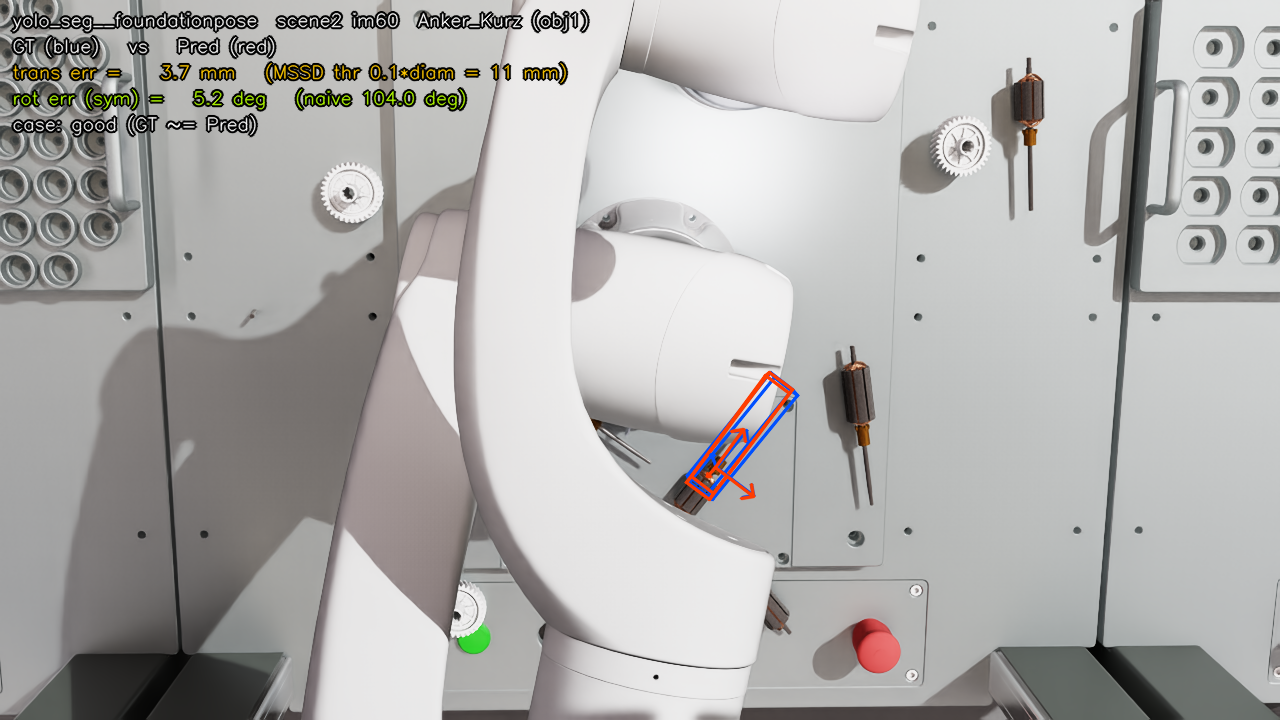
\includegraphics[width=\textwidth]{t175_3_good_4mm.png}
  \caption{gut, 3,7\,mm}
\end{subfigure}\hfill
\begin{subfigure}[b]{0.32\textwidth}
  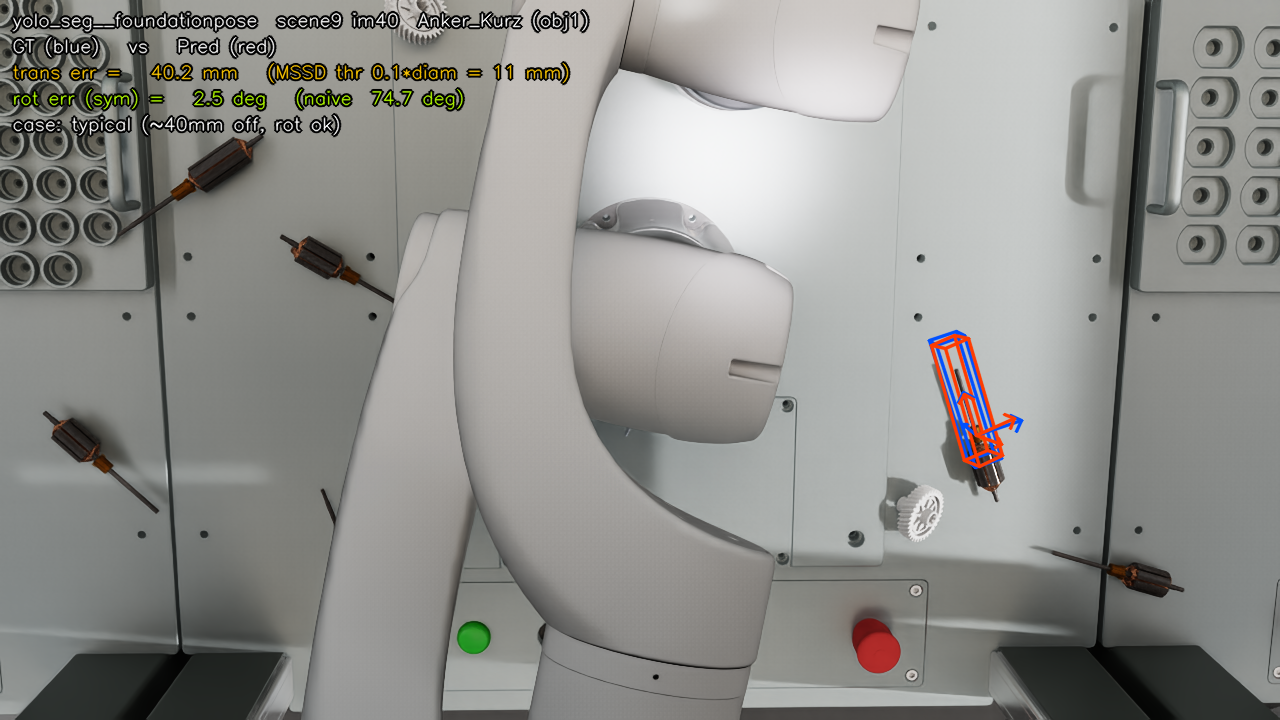
\includegraphics[width=\textwidth]{t175_1_typical_40mm.png}
  \caption{typisch, 40,2\,mm}
\end{subfigure}\hfill
\begin{subfigure}[b]{0.32\textwidth}
  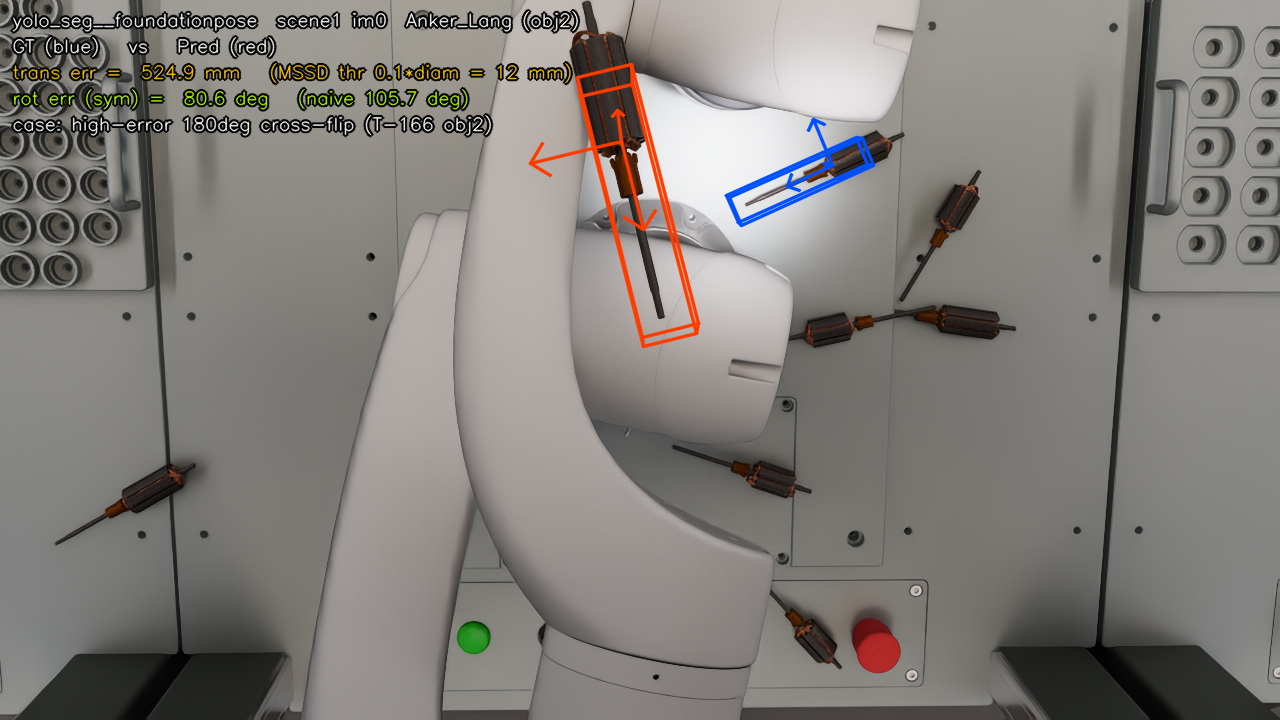
\includegraphics[width=\textwidth]{t175_2_highflip_525mm.png}
  \caption{starker Fehler, 524,9\,mm}
\end{subfigure}
\caption{Anschauliche Fehlerbilder des Tiefenwegs. Die Referenz ist blau, die
Schätzung rot, jeweils als in das Bild projizierte Box des Teils. Der große
unbereinigte Drehwert zeigt die korrekt herausgerechnete Symmetrie; die deutliche
Trennung der Boxen im Fehlerfall macht sichtbar, warum das dreidimensionale Maß
einbricht, während das zweidimensionale Maß hält.}
\label{fig:overlays}
\end{figure}

Ergänzend wurden mehrere Stellhebel geprüft und verworfen, weil sie keine
Verbesserung brachten. Eine Verringerung der Verfeinerungsschritte von
FoundationPose kostete je Schritt rund zwei Prozentpunkte Genauigkeit, sodass die
ursprüngliche Zahl der Schritte das Optimum bleibt. Eine Vergrößerung der
Bildausschnitte für GDRNPP verschlechterte das Ergebnis von 0,885 auf 0,856, weil
das Verfahren den Ausschnitt bereits selbst angemessen wählt. Diese Ergebnisse
stützen die Aussage, dass die Genauigkeit der trainingsfreien Tiefenverfeinerung
auf den bekannten Ankern eine Grenze erreicht hat.

\section{Vergleich der getrennten Wege}
\label{sec:vergleich}

Die getrennte Optimierung beider Wege führt zu einem klaren Ergebnis, das
Tabelle~\ref{tab:getrennt} zusammenfasst. Über alle untersuchten Kombinationen
stieg der mittlere Average Recall von 0,49 auf 0,85. Der genaueste praktisch
einsetzbare Weg ist der Farbweg mit Pipeline~A und einem Average Recall von 0,886.
Der absolut genaueste Weg ist der Tiefenweg mit FoundationPose und 0,968, der
allerdings nur auf idealer Tiefe gilt und unter einer nicht-kommerziellen Lizenz
steht. Die beste lizenzfreie Tiefenvariante, GigaPose im Tiefenmodus, liegt mit
0,838 unter dem Farbweg.

\begin{table}[H]
\caption{Vergleich der getrennten Wege, Average Recall auf den Ankerklassen über
jeweils 100 Szenen, Absturzrate null Prozent. Aufgeführt ist je Verfahrensfamilie
die stärkste Kombination.}
\label{tab:getrennt}
\centering
\small
\begin{tabularx}{\textwidth}{l l c X}
\toprule
\textbf{Kombination (Erkennung und Lage)} & \textbf{Modalität} & \textbf{AR} & \textbf{Einordnung} \\
\midrule
YOLO-OBB und FoundationPose & RGB-D & 0,968 & absolute Spitze, nicht kommerziell, rund 8\,s je Bild \\
YOLO-OBB und GDRNPP (Pipeline~A) & RGB & 0,886 & genaueste einsetzbare Variante \\
YOLO-OBB und GigaPose-3D & RGB-D & 0,838 & beste lizenzfreie Tiefenvariante \\
YOLO-OBB und GigaPose-2D & RGB & 0,636 & Farbe grob, mit Tischebenenbedingung \\
\midrule
\multicolumn{2}{l}{\textit{Mittel über alle Kombinationen}} & 0,49 auf 0,85 & nach den Datenkorrekturen \\
\bottomrule
\end{tabularx}
\end{table}

Daraus folgt das Fazit der getrennten Betrachtung. Beide Wege funktionieren für
sich genommen gut, aber nicht unter denselben Bedingungen gleichzeitig. Der
Tiefenweg ist genauer, wo verlässliche Tiefe vorliegt. Genau dort versagt er
jedoch im realen Betrieb, denn die Tiefenkamera projiziert ein Infrarot-Muster,
und der Roboterarm wirft einen Infrarot-Schatten auf den Tisch. In diesem Schatten
gibt es keine Tiefe, und ein Teil ist dort mit dem Tiefenweg nicht schätzbar,
während der Farbweg unbeeinträchtigt weiterarbeitet. Ein einziges, fest gewähltes
Verfahren ist damit nicht optimal. Wer überall den Tiefenweg wählt, ist im
Schatten blind; wer überall den Farbweg wählt, verschenkt außerhalb des Schattens
die genauere Tiefe. Die sinnvolle Konsequenz ist eine örtliche Entscheidung je
Bauteil, und genau diese setzt die Lösung im folgenden Kapitel um.

% ====================================================================
\chapter{Lösung: modulares System mit Expertenauswahl}
\label{ch:loesung}
% ====================================================================

\section{Grundidee}
\label{sec:loesung-idee}

Die Lösung verbindet beide Wege zu einem modularen System, das für jedes Bauteil
den jeweils geeigneten Weg auswählt. Ein solches Vorgehen wird in der
Bildverarbeitung als Expertenauswahl bezeichnet, weil mehrere spezialisierte
Verfahren bereitstehen und ein Auswahlschritt das passende auswählt. Die Auswahl
richtet sich nach der Lage des Bauteils auf dem Tisch. Liegt es im
Infrarot-Schatten des Arms, wo keine Tiefe verfügbar ist, übernimmt der Farbweg;
liegt es außerhalb, übernimmt der genauere Tiefenweg. Voraussetzung dafür ist,
dass das System weiß, wo der Schatten auf dem Tisch liegt. Diese Schattenkarte
wird vorab geometrisch berechnet.

\section{Berechnung des Infrarot-Schattens}
\label{sec:raytracing}

Der Schatten hängt allein von der Geometrie der Zelle ab, also von der Position
der Kameras, der Stellung des Arms und der Lage der Tischfläche. Die Farbkamera
sitzt in Weltkoordinaten bei 450, 88 und 1100 Millimeter, die Infrarot- und
Tiefenkamera 15 Zentimeter links davon bei 300, 88 und 1100 Millimeter. Die
Tischfläche erstreckt sich von 57 bis 783 Millimeter in der einen und von 42 bis
537 Millimeter in der anderen Richtung. Als Schattenwerfer dient das vollständige
Modell der Zelle mit dem Arm in seiner Arbeitsstellung.

Zur Berechnung der Schattenfläche werden von den Lichtquellen Strahlen auf das
Raster der Tischfläche geschossen und es wird geprüft, ob sie zuvor auf das
Zellenmodell treffen. Hierfür wird ein Standardverfahren der Computergrafik zur
Berechnung des Schnittpunkts zwischen einem Strahl und einer Dreiecksfläche
verwendet \cite{mollertrumbore1997}. Maßgeblich für die fehlende Tiefe ist eine
doppelte Bedingung. Tiefe fehlt dort, wo entweder der Projektor der Tiefenkamera
verdeckt ist, was den eigentlichen Infrarot-Schatten ausmacht, oder die Farbkamera
nicht hinsieht, was den Sichtschatten ausmacht. Daraus ergeben sich drei
Bereiche, die Tabelle~\ref{tab:zonen} aufführt und die Abbildung~\ref{fig:shadow}
im Schnitt darstellt. Der Infrarot-Schatten bedeckt rund 43 Prozent der
Tischfläche, der Sichtschatten rund 39 Prozent. Entscheidend für die Auswahl ist
die Schnittmenge, in der zwar die Tiefe fehlt, die Farbkamera aber noch hinsieht.
Dieser Bereich umfasst rund 13 Prozent der Tischfläche und bildet die Fläche, in
der das System auf den Farbweg umschalten muss. Da die Lichtquelle links steht,
fällt der Schatten nach rechts und bildet im Wesentlichen einen Streifen am
rechten Tischrand. Das Ergebnis dieser Berechnung, die Umrisse der Bereiche, wird
als zentrale Schattenkarte gespeichert und vom System geladen. Ändert sich die
Position von Kamera oder Arm, wird die Berechnung erneut ausgeführt.

\begin{table}[H]
\caption{Bereiche auf der Tischfläche aus der Schattenberechnung.}
\label{tab:zonen}
\centering
\small
\begin{tabular}{l c c}
\toprule
\textbf{Bereich} & \textbf{Fläche} & \textbf{Anteil} \\
\midrule
Infrarot-Schatten (gesamt)        & 1569\,$\text{cm}^2$ & 42,9\,\% \\
Sichtschatten (Farbkamera verdeckt) & 1435\,$\text{cm}^2$ & 39,3\,\% \\
Auswahlbereich für den Farbweg     & 485\,$\text{cm}^2$  & 13,3\,\% \\
\bottomrule
\end{tabular}
\end{table}

\begin{figure}[H]
\centering
\begin{tikzpicture}[font=\small, >={Stealth[length=2mm]}]
  % Tisch
  \draw[thick] (0,0) -- (10,0);
  \node[anchor=north east] at (10,-0.05) {\scriptsize Tischfläche};
  % Quellen
  \node[circle, fill=shadowred, inner sep=1.7pt, label={[shadowred]above:{\scriptsize IR-Projektor}}] (ir) at (1.6,4.4) {};
  \node[circle, fill=rgbblue, inner sep=1.7pt, label={[rgbblue]above:{\scriptsize Farbkamera}}] (rgb) at (8.6,4.4) {};
  % Arm als Block auf dem Tisch
  \fill[gray!45, draw=black!55] (4.2,0) rectangle (5.2,2.4);
  \node[gray!20] at (4.7,1.2) {\scriptsize Arm};
  % Schattengrenzen vom IR-Projektor ueber die Armkanten auf den Tisch
  \draw[shadowred, densely dashed] (ir) -- (4.2,2.4) -- (5.55,0);
  \draw[shadowred, densely dashed] (ir) -- (5.2,2.4) -- (7.55,0);
  % IR-Schatten auf dem Tisch (kein Tiefensignal)
  \fill[shadowred!22] (5.55,0) rectangle (7.55,0.32);
  % davon der Auswahlbereich (Farbkamera sieht noch hin)
  \fill[rgbblue!35, draw=rgbblue] (5.55,0) rectangle (7.0,0.32);
  % Sichtlinie der Farbkamera in den Auswahlbereich
  \draw[rgbblue, densely dotted] (rgb) -- (6.3,0.1);
  % Beschriftungen
  \node[shadowred, anchor=west, font=\scriptsize] at (7.65,0.55) {Infrarot-Schatten};
  \node[shadowred, anchor=west, font=\scriptsize] at (7.65,0.18) {(keine Tiefe)};
  \node[rgbblue, anchor=north, font=\scriptsize, align=center] at (6.25,-0.15) {Auswahlbereich:\\Farbkamera sieht hier noch};
\end{tikzpicture}
\caption{Schattenwurf im Schnitt. Der Infrarot-Projektor steht links, sein Strahl
wird vom Arm blockiert, sodass auf dem Tisch rechts ein Bereich ohne Tiefe
entsteht. In dem Teil dieses Bereichs, den die rechts stehende Farbkamera noch
einsieht, schaltet das System auf den Farbweg um.}
\label{fig:shadow}
\end{figure}

\section{Auswahl ohne Tiefe}
\label{sec:routing}

Die Besonderheit der Lösung ist, dass die Auswahl ohne Tiefe getroffen werden
muss, denn im Schatten ist die Tiefe gerade nicht verfügbar. Für jedes erkannte
Bauteil läuft daher der in Abbildung~\ref{fig:moe-arch} dargestellte Ablauf. Der
Detektor liefert die Bildposition des Bauteils. Aus dieser Bildposition wird der
zugehörige Sehstrahl mit der bekannten Tischebene geschnitten, was die vermutete
Aufstandsstelle des Teils in Weltkoordinaten ergibt. Diese Stelle wird
geometrisch und damit ohne jede Tiefeninformation bestimmt. Anschließend prüft das
System, ob die Stelle im Auswahlbereich liegt. Liegt sie darin, übernimmt der
Farbweg mit GDRNPP; liegt sie außerhalb, übernimmt der Tiefenweg mit GigaPose im
Tiefenmodus, wobei FoundationPose wegen seiner Lizenz nur als Vergleichsmaßstab
dient. Zusätzlich gibt es eine fähigkeitsbasierte Auswahl: Bauteilklassen, für die
noch keine Tiefenvorlagen vorliegen, etwa das Zahnrad, laufen unabhängig von ihrer
Lage stets über den Farbweg. So funktioniert jede Klasse an jeder Stelle des
Tisches.

\begin{figure}[H]
\centering
\begin{tikzpicture}[node distance=6mm and 10mm]
  \node[pipe]                      (det) {Bildposition\\des Bauteils};
  \node[pipe, right=of det]        (ray) {Schnitt mit\\der Tischebene};
  \node[dec,  right=of ray]        (pip) {im Auswahl-\\bereich?};
  \node[pipeR, above right=3mm and 11mm of pip] (rgb)  {Farbweg\\GDRNPP};
  \node[pipeD, below right=3mm and 11mm of pip] (rgbd) {Tiefenweg\\GigaPose-3D};
  \node[pipe, right=24mm of pip]   (out) {Lage des\\Bauteils};
  \draw[flow] (det) -- (ray);
  \draw[flow] (ray) -- (pip);
  \draw[flow] (pip) -- node[above left, font=\scriptsize]{ja} (rgb);
  \draw[flow] (pip) -- node[below left, font=\scriptsize]{nein} (rgbd);
  \draw[flow] (rgb)  -| (out);
  \draw[flow] (rgbd) -| (out);
\end{tikzpicture}
\caption{Auswahl ohne Tiefe. Die Lage des Bauteils wird rein geometrisch über die
Tischebene bestimmt; je nach Lage im Schattenbereich wählt das System den Farb-
oder den Tiefenweg.}
\label{fig:moe-arch}
\end{figure}

\section{Aufbau des Systems}
\label{sec:impl}

Das System ist aus eigenständigen Diensten aufgebaut, die sich frei kombinieren
lassen. Ein zentraler Server bedient den Live-Betrieb des Farbwegs unmittelbar und
leitet die übrigen Kombinationen an ein Bindeglied weiter, das die einzelnen
Modelldienste anspricht. Jede Pipeline ist zweistufig aufgebaut, mit einem Schritt
für die Erkennung und einem Schritt für die Lageschätzung. Dadurch lassen sich
Erkennung und Lageschätzung frei zusammenstellen. Formal ergeben drei
Erkennungs- und vier Lageverfahren zwölf sinnvolle Kombinationen. Das modulare
System mit Expertenauswahl steht bewusst neben dieser festen Auswahl und stellt
eine eigenständige Sonderpipeline dar.

Damit die Wirkung des Schattens nicht nur an realen Bildern behauptet, sondern
nachvollziehbar belegt werden kann, wird sie im Simulationsbetrieb vollständig
nachgebildet. Dazu wird die gerenderte Tiefe innerhalb des Infrarot-Schattens vor
der Lageschätzung ausgeblendet, was rund 76000 Bildpunkte je Bild betrifft. Der
Tiefenweg erlebt in der Simulation damit dieselbe Blindheit wie in der realen
Anlage. Auf demselben Bild wird zusätzlich ein reiner Tiefenweg als Vergleich
ausgewertet, dessen Ergebnis Abschnitt~\ref{sec:moe-ergebnis} darstellt.

Zur Anschauung stellt ein eigener Bereich der Benutzeroberfläche die
Schattenfläche auf dem dreidimensionalen Tisch dar, zusammen mit dem Lichtkegel
der Infrarotquelle, und zeigt nach jedem Lauf, wie viele Teile über den Farb- und
wie viele über den Tiefenweg geschätzt wurden.

\section{Wirksamkeit der Lösung}
\label{sec:moe-ergebnis}

Der direkte Vergleich auf einem Testbild mit ausgeblendeter Tiefe im Schatten
belegt die Wirkung der Lösung, wie Tabelle~\ref{tab:moe-ab} zeigt. Für ein Teil
innerhalb des Schattenbereichs verringert die Auswahl des Farbwegs den Fehler von
424,6 Millimeter, den der reine Tiefenweg im Schatten erleidet, auf 3,4
Millimeter. Für ein Teil außerhalb des Bereichs bleibt der Tiefenweg unverändert,
mit 16,2 gegenüber 9,4 Millimeter, da die Auswahl dort nicht eingreift. Das
modulare System holt damit die Verluste im Schatten zurück, ohne die Stärke des
Tiefenwegs außerhalb des Schattens aufzugeben.

\begin{table}[H]
\caption{Wirksamkeit der Lösung anhand eines Testbildes mit im Schatten
ausgeblendeter Tiefe. Angegeben ist der Lagefehler. Die Auswahl rettet das Teil im
Schatten; außerhalb bleibt der Tiefenweg unverändert.}
\label{tab:moe-ab}
\centering
\small
\begin{tabular}{l l c c}
\toprule
\textbf{Teil} & \textbf{Lage} & \textbf{mit Auswahl} & \textbf{nur Tiefenweg} \\
\midrule
Anker kurz & im Schatten   & Farbweg, 3,4\,mm   & 424,6\,mm \\
Anker lang & außerhalb     & Tiefenweg, 16,2\,mm & 9,4\,mm \\
\bottomrule
\end{tabular}
\end{table}

\section{Einordnung und Grenzen}

Die Ergebnisse sind unter mehreren Vorbehalten zu lesen. Die Bewertung beruht auf
der korrigierten Tiefe aus der Simulation, die nahezu ideal ist. Reale Tiefe auf
glänzendem Metall ist verrauscht, was der ursprüngliche Grund für die Wahl des
reinen Farbwegs war. Eine Prüfung an einem kleinen realen Tiefendatensatz steht
aus und ist die wichtigste offene Frage. Das genaueste Tiefenverfahren ist nur
nicht-kommerziell nutzbar und dient daher allein als Vergleichsmaßstab; die
einsetzbare Tiefenvariante bleibt GigaPose im Tiefenmodus. Die berechnete
Schattenfläche gilt nur für die konkrete Stellung von Kamera und Arm und muss bei
einer Änderung neu bestimmt werden; auch der Abgleich der berechneten mit der
realen Schattenfläche steht noch aus. Schließlich treten bei teilweiser Sicht
echte Mehrdeutigkeiten der Drehlage der Anker auf, die kein Weg allein auflöst.

% ====================================================================
\chapter{Ausblick}
% ====================================================================

Die nächsten Schritte ergeben sich unmittelbar aus den genannten Grenzen. An
erster Stelle steht die Prüfung an realen Daten. Ein kleiner Datensatz mit echter
Tiefe sollte durch beide Wege gemessen und die reale Schattenfläche mit der
berechneten verglichen werden. Erst dies beziffert, wie groß der Vorteil des
Tiefenwegs außerhalb des Schattens unter realem Rauschen tatsächlich ausfällt. An
zweiter Stelle steht die Vervollständigung des Tiefenwegs, indem für das Zahnrad
Tiefenvorlagen erstellt werden, sodass auch diese Klasse außerhalb des Schattens
über den Tiefenweg geschätzt werden kann. An dritter Stelle steht die
Übertragbarkeit. Der modulare Aufbau erlaubt es, neue Bauteile und neue Verfahren
ohne strukturelle Änderung aufzunehmen, und in Verbindung mit den trainingsfreien
Verfahren ist die Erweiterung auf beliebige Konstruktionsteile der natürliche
nächste Ausbauschritt. Die Kernaussage der Arbeit bleibt bestehen: Farbbild und
Tiefenbild sind keine Konkurrenten, sondern örtlich ergänzende Experten, und eine
geometrisch gesteuerte Auswahl nutzt beide dort, wo sie jeweils stark sind.

% Schlussteil im backmatter.
\backmatter

\tocloftpagestyle{scrheadings}
%! Abbildungsverzeichnis
\listoffigures

\newpage
%! Tabellenverzeichnis
\listoftables

\newpage
%! Listingverzeichnis
\lstlistoflistings

% Literaturverzeichnis
	\cleardoublepage
	\phantomsection
	\addcontentsline{toc}{chapter}{\bibname}
%! Name der .bib-Datei angeben (Zotero-Export).
	\bibliography{Literaturfile}

\clearpage{\pagestyle{scrheadings}\cleardoublepage}

%! Anhang
\renewcommand{\thefigure}{A.\arabic{figure}}
\renewcommand{\thetable}{A.\arabic{table}}
\renewcommand{\thelstlisting}{A.\arabic{lstlisting}}

\setcounter{figure}{0}
\chapter{Anhang}
\quad  \addtocounter{page}{-1}
% Anhang wird von der normalen Nummerierung ausgenommen.
% Beschriftungen erfolgen mit Abbildung, Tabelle und A.x.

\end{document}
